\documentclass[14pt,a4paper]{extarticle}
\usepackage[T2A]{fontenc}
\usepackage[utf8]{inputenc}
\usepackage[russian]{babel}
\usepackage{graphicx,epstopdf}
\usepackage{amsfonts,amssymb,amscd,amsmath}
\usepackage[left=2.5cm, right=2.5cm, top=2.7cm, bottom=2cm]{geometry}

\usepackage[usenames]{color}
\usepackage{colortbl}

\begin{document}
	
	\title {Баг-трекер}
	
	\section {Термины}
	\begin{enumerate}
		\item {\bf Баг-трекер, трекер, система отслеживания ошибок, система} --- прикладная программа, разработанная с целью помочь разработчикам программного обеспечения учитывать и контролировать ошибки, найденные в программах, пожелания пользователей, а также следить за процессом устранения этих ошибок и выполнения или невыполнения пожеланий.
		
		\item {\bf Проект} --- основная структурная единица.
		
		\item {\bf Задача} --- задание, требующие выполнения.
		
		\item {\bf Администратор} --- лицо, занимающеесяся непосредственным обслуживанием системы, обеспечивающее её нормальное функционирование без сбоев и ошибок.
		
		\item {\bf Авторизовавшийся пользователь, пользователь} --- лицо, успешно прошеднее процедуру авторизации и обладающие возможностью работы с проектами в рамках ролей, установленных для него в проектах.
		
		\item {\bf Гость} --- лицо, не прошедшее процедуру авторизации. Не имеет возможности работать с системой.
		
		\item {\bf Главный разработчик проекта} --- лицо, отвечающее за распределение задач по своему проекту.
		
		\item {\bf Разработчик} --- лицо, отвечающее за выполнение назначенных на него задач по своему проекту.
		
		\item {\bf Заказчик} --- лицо, ставящее задачи разработчикам проекта.
		
		\item {\bf Форматирование текста} --- выделение частей текста полужирным, курсивом и/или подчеркиванием.
		
		\item {\bf Оповещения} --- сообщения, приходящие пользователю на почту (указанную при регистрации).
	\end{enumerate}
	
	
	\section {Общие положения}
	\begin{enumerate}
		\item {\bfПроект}
		\begin{enumerate}
			\item Каждый проект характеризуется следующими полями:
			\begin{itemize}
				\item название проекта
				\item описание (с возможностью форматирования текста)
				\item список пользователей, относящихся к проекту
				\item главный разработчкик проекта
				\item заказчик проекта
			\end{itemize}
			
			\item Поддержка нескольких проектов одновременно.
			
			\item Проекты могут иметь следующие статусы:
			\begin{itemize}
				\item активен -- проект находится в активной стадии разработки
				\item завершен -- проект завершен, разработка прекращена
			\end{itemize}
			
			\item Проекты включают в себя задачи.
			
			\item В решении задач проекта может участвовать только пользователь, относящийся к данному проекту.
			
		\end{enumerate}
		
		\item {\bfЗадача}
		\begin{enumerate}
			\item Задача описывается следующими полями:
			\begin{itemize}
				\item название задачи
				
				\item описание (с возможностью форматирования текста)
				
				\item дата создания (выставляется {\bfавтоматически} при создании задачи)
				
				\item дата крайнего срока (опционально, может не указываться, в таком случае у задачи нет конкретного времени выполнения)
				
				\item статус задачи
				\begin{itemize}
					\item открыта -- задача требует решения
					\item решается -- на данный момент задача взята одним из разработчиков
					\item решена -- разработчик, отвественный за задачу счел решение готовым
					\item не решаем -- задача не будет решаться
					\item закрыта -- вопросы по данной задаче считаются полностью решенными
				\end{itemize}
				Схема переходов представлена в следующей части.
				
				\item приоритет задачи
				\begin{itemize}
					\item нормальный
					\item важный
					\item не важный
				\end{itemize}
			\end{itemize}
			
			\item К задаче могут быть приложены документы. Размер одного документа не должен превышать 5MB. Количество приложений к задаче неограничено. Ограничение на тип файла не накладывается.
			
			\item Обсуждение задачи и лента изменений представляет собой <<ленту новостей>>. Обсуждение задачи -- комментарии пользователей системы. Лента изменений -- комментарии системы. Система оставляет сообщения об изменении статуса задачи.
		\end{enumerate}
		
		\item {\bfПользователи}
		\begin{enumerate}
			\item {\bfПо правам доступа к возможностям системы}
			\begin{itemize}
				\item {\bfадминистратор системы}
				Количество администраторов в системе неограничено. Снять с должности администратора может лишь ругой администратор.
				\begin{itemize}
					\item {\it Функции}
					\begin{itemize}
						\item регистрирует пользователей
						\item создает / удаляет проекты
						\item удаляет комментарии пользователей
						\item назначает на проект главных разработчиков
						\item назнчает заказчика на проект
					\end{itemize}
					
					\item {\it Оповещения}
					\begin{itemize}
						\item не получает
					\end{itemize}
				\end{itemize}
				
				\item {\bfавторизовавшийся пользователь}
				
				\item {\bfгость}
				
			\end{itemize}
			
			\item {\bfПо ролям внутри каждого проекта в отдельности}
			Пользователь может обладать различными ролями в различных проектах. Внутри конкретного проекта роль каждого пользователя однозначна. (+ про администратора системы в терминологии проектов). Все описанные функции/возможности ролей доступны только если пользователь обладет этой ролью в конкретном проекте.
			\begin{itemize}
				\item {\bf главный разработчик проекта} -- уникален для каждого проекта
				\begin{itemize}
					\item {\it Функции}
					\begin{itemize}
						\item собирает<<команду проекта>>, заносит пользователей в проект в качестве разработчиков, добавляет и удаляет разработчиков из проекта
						\item создает задачи
						\item принимает созданным им задачи
						\item ставит задачи на себя и на разработчиков проекта
						\item изменяет статусы задач
					\end{itemize}
					Задачи, созданные заказчиком проекта, назначаются на главного разработчика проекта.
					
					\item {\it Оповещения}
					\begin{itemize}
						\item создан проект и он (данный пользователь) назначеен главным разработчиком этого проекта
						
						\item изменен статус любой задачи в проекте (где он главный разработчик)
						
						\item изменен статус проекта (где он главный разработчик)
						
						\item приближается время завершения задачи (за 3 дня), на которую он назначен
						
						\item просрочена задача, на которую он назначен
						
						\item изменился исполнитель задачи, которую он создал
						
						\item снят с задачи
					\end{itemize}
				\end{itemize}
				
				\item {\bfразработчик}
				\begin{itemize}
					\item {\it Функции}
					\begin{itemize}
						\item создает задачи
						\item ставит задачи на себя и на разработчиков проекта (в том числе и на главного разработчика)
						\item изменяет статусы задач
						\item принимает созданные им задачи
					\end{itemize}
					
					\item {\it Оповещения}
					\begin{itemize}
						\item назначен на проект
						\item удален из проекта
						\item изменен статус задачи, на которую он назначен
						\item приближается время завершения задачи (за 3 дня), на которую он назначен
						\item просрочена задача, на которую он назначен
						\item изменился исполнитель задачи, которую он создал
					\end{itemize}
					
				\end{itemize}
				
				\item {\bfзаказчик}
				\begin{itemize}
					\item {\it Функции}
					\begin{itemize}
						\item создает задачи ({\bfавтоматически} назначаются на главного разработчкиа проекта)
						\item изменяет статусы задач, которые создал
						\item принимает созданным им задачи
					\end{itemize}
					
					\item {\it Оповещения}
					\begin{itemize}
						\item создан проект, где он заказчик
						\item изменен статус проекта, где он заказчик
						\item изменился исполнитель задачи, которую он создал
					\end{itemize}
					
				\end{itemize}
				
				\item {\bfпользователь, не относящийся к проекту}
				Данный пользователь никак не задействован в проекте. Видит общую информацию о проекте. Название, описание, главного разработчика, заказчика и список задач.
			\end{itemize}
		\end{enumerate}
		
%		\item {\bfОповещения}
%		\begin{enumerate}
%			\item Приходят в следующих случаях:
%			\begin{itemize}
%				\item выполнена регистрация в системе -- всем пользователям
%				\item создан проект -- заказчику
%				\item изменен статус задачи -- пользователь, на которого назначена задача
%				\item изменен статус проекта -- все пользователи, имеющие отношение к данному проекту (заказчик, менеджер проекта, разработчик)
%				\item приближается время завершения задачи -- пользователь, на которого назначена задача
%				\item задача просрочена -- пользователь, на которого назначена задача
%			\end{itemize}
%		\end{enumerate}
		
		\item {\bfФильтры задач}
		\begin{enumerate}
			\item  Возможны следующие фильтры:
			\begin{itemize}
				\item по исполнителю
				\item по дате создания
				\item по статусу
				\item по последней активности
				\item проваленные по срокам
			\end{itemize}
			
			\item Различные комбинации фильтров
		\end{enumerate}
		
	\end{enumerate}
	
%	\section {Действия в системе. Должно быть пунктами, с описанием всех сопутствующий действия. Вроде <<отправка уведомления на почту>>}
%	\begin{enumerate}
%		\item {\bfСоздание проекта}
%		
%		При создании проекта администратор указывает название, описание, главный разработчик и заказчик проекта. Все пункты, кроме описания, являются обязательными
%		
%		\item {\bfРегистрация пользователя}
%		
%		Регистрацию пользователей осуществляет администратор. При регистрации пользователя указывается e-mail и имя пользователя. Пароль генерируется автоматически. На указанный e-mail высылается сгенерированный пароль. Администратор не видит пароль.
%		
%		 \item {\bfАвторизация в системе}
%		 
%		 Для авторизации в системе используется пара email-пароль.
%	\end{enumerate}
	
	
	%\section {Макеты}
	\section {Детали реализации}
	\begin{enumerate}
		\item{\bfСредства разработки}
		\begin{enumerate}
			\item {\bfСерверная часть}
			\begin{enumerate}
				\item ASP.NET
			\end{enumerate}
			
			\item {\bfКлиентская часть}
			\begin{enumerate}
				\item AngularJS
			\end{enumerate}
		\end{enumerate}
		
		\item{\bfБаза данных}
			В разработке...
			
		\item{\bfСхема переходов для статусов задачи}
			\begin{center}
				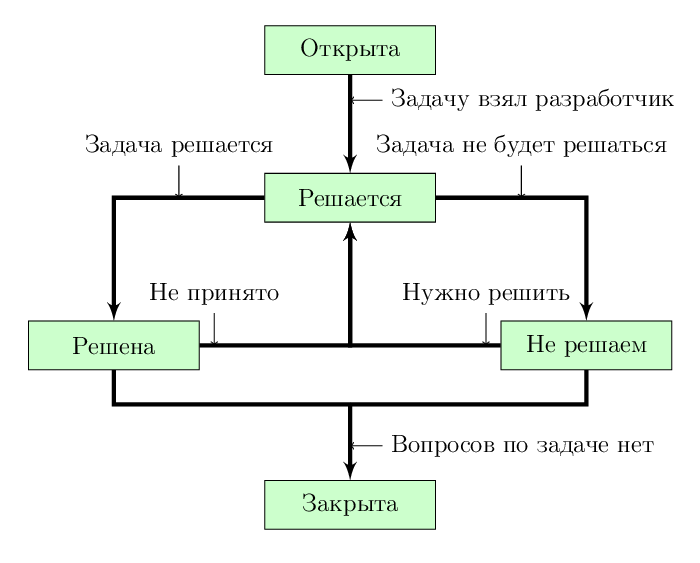
\includegraphics[scale=0.5]{res/TransitionScheme/TransitionScheme.png} 
			\end{center}
			
		\item{\bfДетальное описание страниц}
			\begin{enumerate}
				\item{\it Страница авторизации}\\
				На этой странице расположены поля для ввода <<E-mail>> и пароля, а также кнопка <<Войти>>. Оба поля являются обязательными для заполнения и помечаются (\textcolor{red}{*}) (красная звездочка).\\
				При нажатии кнопки <<Войти>> происходит валидация. В случае если значение введено не верно поле подсвечивается красным появляется надпись <<<значение> введено не верно>> и фокус переводится на поле, где совершена ошибка. Если ни каких ошибок не возникает, то переходим на страницу проектов.
				
				\item{\it Проекты}\\
				На странице <<Проект>> расположена кнопка <<Добавить проект>>, которая доступна только для пользователя с ролью <<Администратор>>.\\
				Так же располагается таблица в которой перечислены все проекты. При нажатии на строчку с проектом переходим на страницу <<Проекта>>. Таблица состоит из нескольких столбцов: название проекта, главный разработчик проекта, заказчик проекта, статус проекта.\\
				\textcolor[rgb]{0.5, 0.5, 0.5}{(описание проекта лучше не вставлять в таблицу, оно большим может быть, но если таблица будет получаться слишком узкой, то придется вставлять и описание)}
				
				\item{\it Добавление проекта}\\
				Данная страница доступна только для пользователя с ролью <<Администратор>>.\\
				На странице <<Добавление проекта>> расположены поля для ввода всех свойств проекта (см. <<Общие положения>>). Поля для выбора главного разработчки и заказчика должны быть реализованы как выпадающие списки.\\
				На данной странице {\bf не добавляются разработчики проекта}.\\
				
				\item {\it Проект (конкретный)}\\
				На странице <<Проекта>> расположены название проекта, описание, список участников проекта (главный разработчик, разработчики, заказчик) и таблица (название задачи, дата создания, дата окончания (может быть пустой!!), создатель задачи, статус и приоритет), в которой перечислены все задачи на данном проекте. Фокус в таблице указывает на первую задачу в списке. Задачи сортируются по <<новизне>>, чем позже создана задаче, тем она выше. Также расположены кнопки <<Добавить>>, <<Изменить>>, <<Просмотр>>, относящиеся к работе с задачами. Панель поиска на которой располагаются поля <<Исполнитель>>, <<Дата создания>>, <<Статус>>, <<Последняя активность>>, <<Проваленные по срокам>> и кнопка <<Найти>>. <<Последняя активность>> -- задачи, у которых последнее сообщение в ленте не позднее 3 дней.\\
				При нажатии на кнопку <<Добавить>> происходит переход на страницу добавления новой задачи.
				При нажатии на задачу (в таблице задач) происходит выделение соответствующей строки.\\
				При нажатии на кнопку <<Изменить>> происходит переход на страницу редактирования выделенной в таблице задачи.\\
				При нажатии на кнопку <<Просмотр>> происходит переход на страницу просмотра выделенной в таблице задачи.\\
				Для пользователя с ролью <<Главный разработчик (данного проекта)>> видна кнопка <<Управление проектом>>, при нажатии на которую происходит переход на страницу управления данным проектом.
				
				\item {\it Добавление задачи}\\
				На странице <<Добавление задачи>> расположены поля: <<Название задачи>>, <<Описание>> (с возможностью форматирования текста) , <<Дата создания>> (выставляется автоматически при создании задачи) , <<Дата крайнего срока>> (опционально, может не указываться, в таком случае у задачи нет конкретного времени выполнения), <<Статус задачи>> (открыта, решается, решена, не решаем, закрыта), <<Приоритет задачи>> (нормальный, важный, не важный). Все поля обязательные к заполнению помечаются (\textcolor{red}{*}) (красная звездочка) (все поля кроме даты крайнего срока).\\
				Кроме того на странице присутствуют кнопки добавления приложение (файлов) и список уже приложенных.\\ 
				Кнопки <<Добавить>> и <<Отмена>>.\\
				При нажатии на кнопку <<Добавить>>, происходит проверка на обязательные поля, если поле не заполнено, то поле подсвечивается красным выдается сообщение об ошибке <<"поле" обязательное к заполнению>> и фокус переводится на поле, где совершена ошибка.\\
				При нажатии на кнопку <<Отмена>>, появляется сообщение <<Введенные данные не будут сохранены. Вы уверены что хотите продолжить?>>\\
				При добавлении задачи появляется системное сообщение в ленте о создании задачи.



			\end{enumerate}
		
	\end{enumerate}
	
\end{document}
